%%================================================
%% Appendix I
%%================================================
\chapter[ภาพประกอบการสำรวจพื้นที่และการติดตั้งต้นแบบ]{\texorpdfstring{ภาคผนวก ฌ\\ภาพประกอบการสำรวจพื้นที่และการติดตั้งต้นแบบ}{Appendix I: Field Photos}}
\label{app:legacy_field_photos}

ภาคผนวกนี้แสดงภาพประกอบจากการสำรวจบริบทพื้นที่ การทดลองติดตั้งอุปกรณ์ และการรับฟังความคิดเห็นจากผู้ดูแล ภาพชุดนี้ใช้เป็นหลักฐานประกอบด้านสภาพแวดล้อมและการออกแบบต้นแบบ ไม่ได้ใช้เป็นหลักฐานว่าระบบผ่านการติดตั้งใช้งานจริงระยะยาวในสถานดูแลผู้สูงอายุ

\begin{figure}[H]
    \centering
    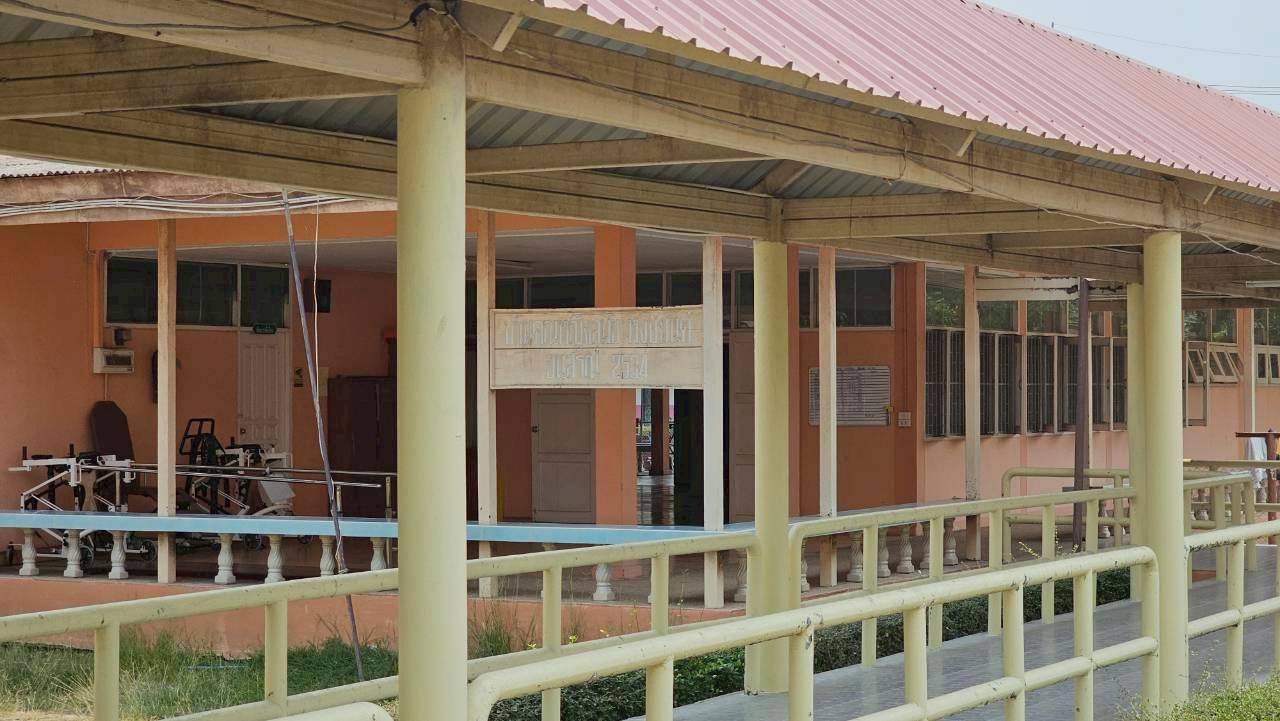
\includegraphics[width=0.82\textwidth]{assets/appendices/legacy-field/facility-building.jpg}
    \caption{ตัวอย่างอาคารและพื้นที่บริการหลักของสถานดูแล}
    \label{fig:appI_building}
\end{figure}
\begin{figure}[H]
    \centering
    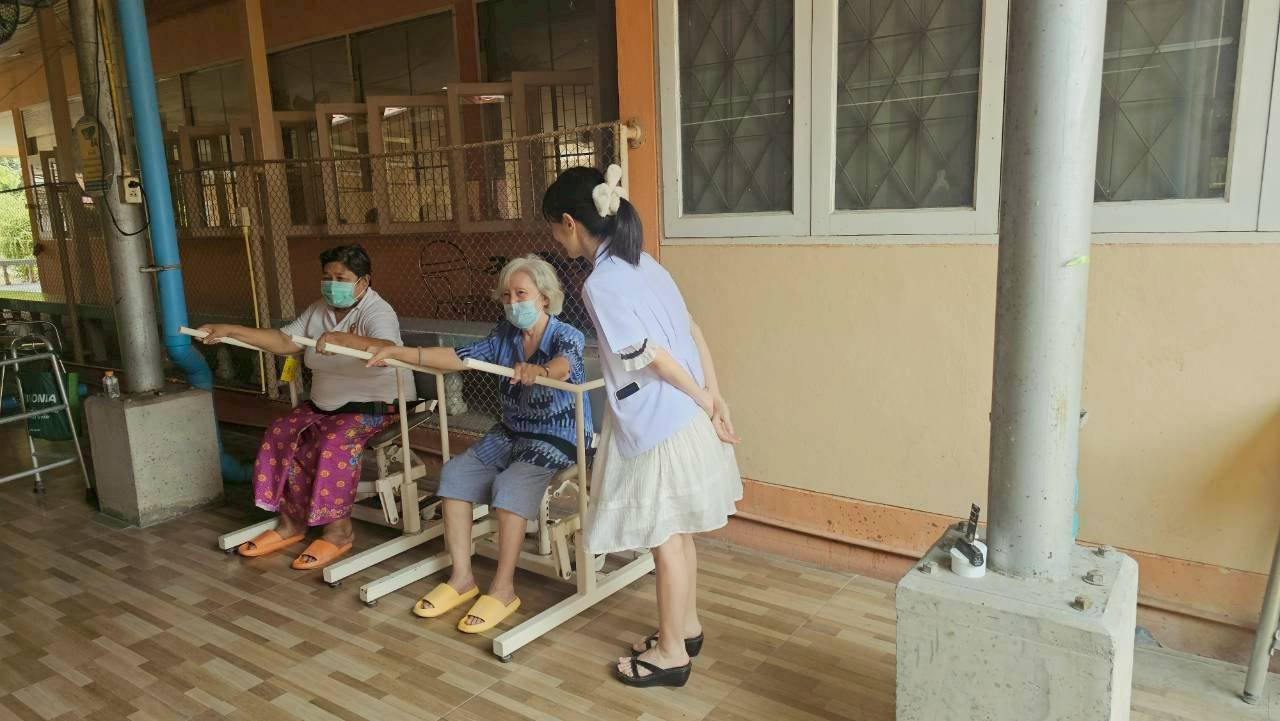
\includegraphics[width=0.82\textwidth]{assets/appendices/legacy-field/node-install-1.jpg}
    \caption{ตัวอย่างการติดตั้ง node อ้างอิงสัญญาณภายในอาคาร}
    \label{fig:appI_node_install1}
\end{figure}

\begin{figure}[H]
    \centering
    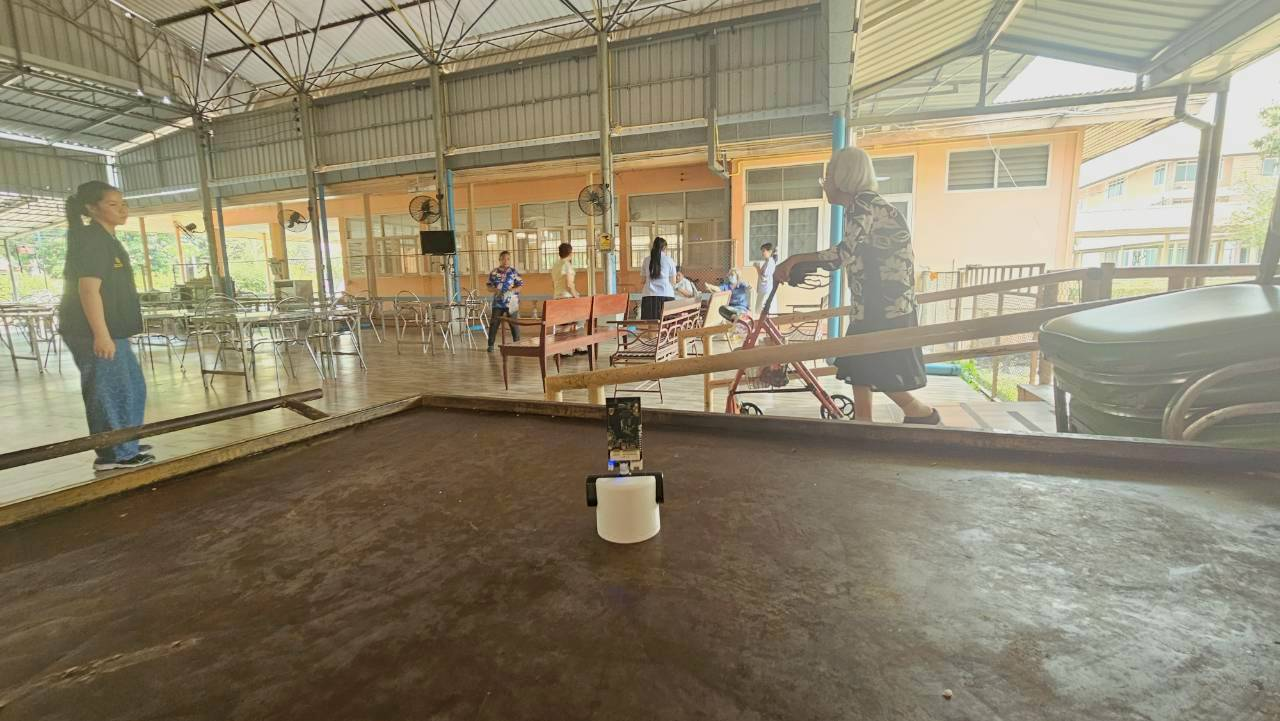
\includegraphics[width=0.82\textwidth]{assets/appendices/legacy-field/node-install-2.jpg}
    \caption{ตัวอย่างตำแหน่งติดตั้ง node ภายในอาคารอีกมุมมองหนึ่ง}
    \label{fig:appI_node_install2}
\end{figure}

\begin{figure}[H]
    \centering
    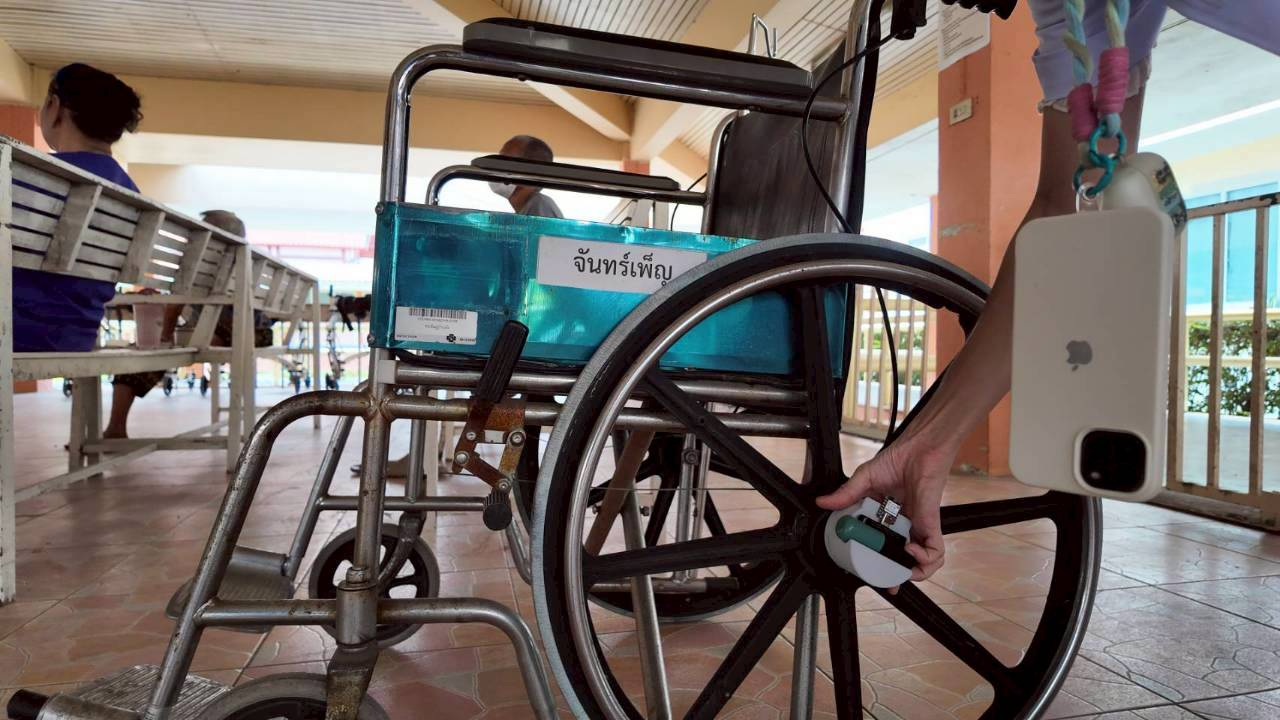
\includegraphics[width=0.82\textwidth]{assets/appendices/legacy-field/wheelchair-install.jpg}
    \caption{ตัวอย่างการติดตั้งอุปกรณ์กับเก้าอี้รถเข็นสำหรับเก็บข้อมูลการเคลื่อนไหว}
    \label{fig:appI_wheelchair_install}
\end{figure}

\begin{figure}[H]
    \centering
    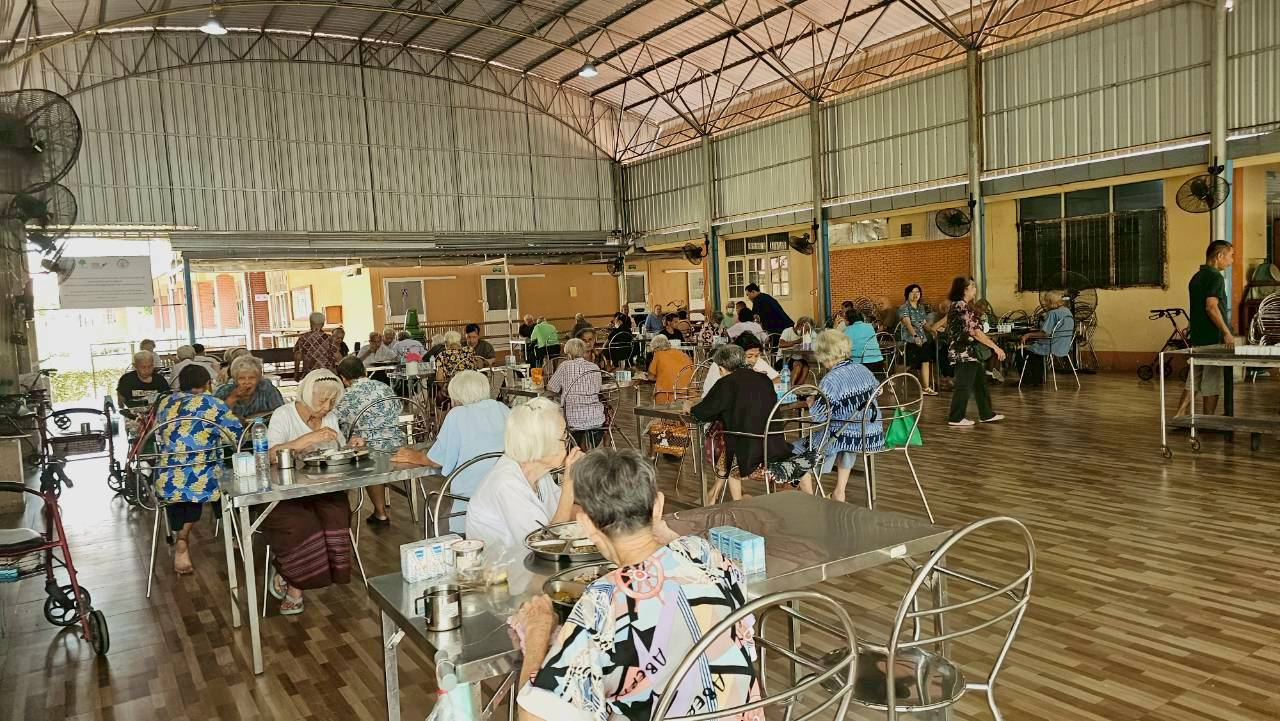
\includegraphics[width=0.82\textwidth]{assets/appendices/legacy-field/elderly-home.jpg}
    \caption{ตัวอย่างบริบทผู้สูงอายุในสถานดูแล}
    \label{fig:appI_elderly_home}
\end{figure}

\begin{figure}[H]
    \centering
    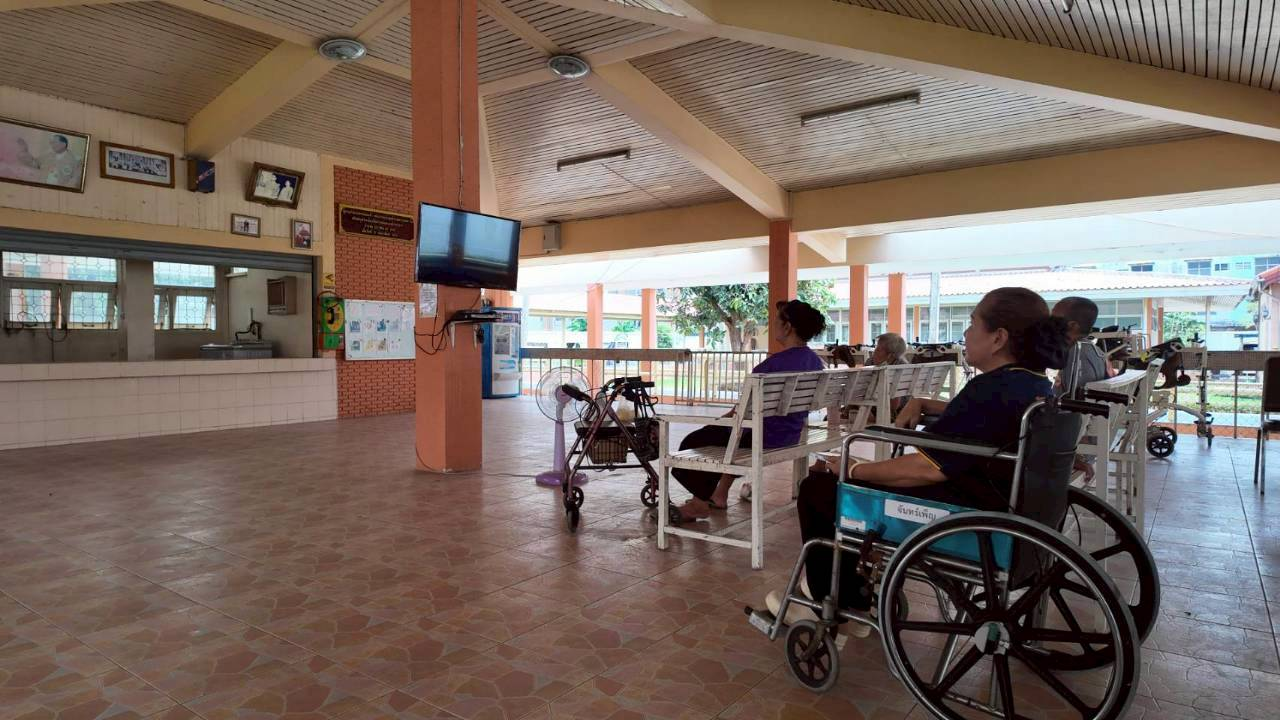
\includegraphics[width=0.82\textwidth]{assets/appendices/legacy-field/elderly-device-use.jpg}
    \caption{ตัวอย่างการใช้งานอุปกรณ์ในบริบทการทดลองต้นแบบ}
    \label{fig:appI_elderly_device_use}
\end{figure}

\begin{figure}[H]
    \centering
    \begin{subfigure}[t]{0.48\textwidth}
        \centering
        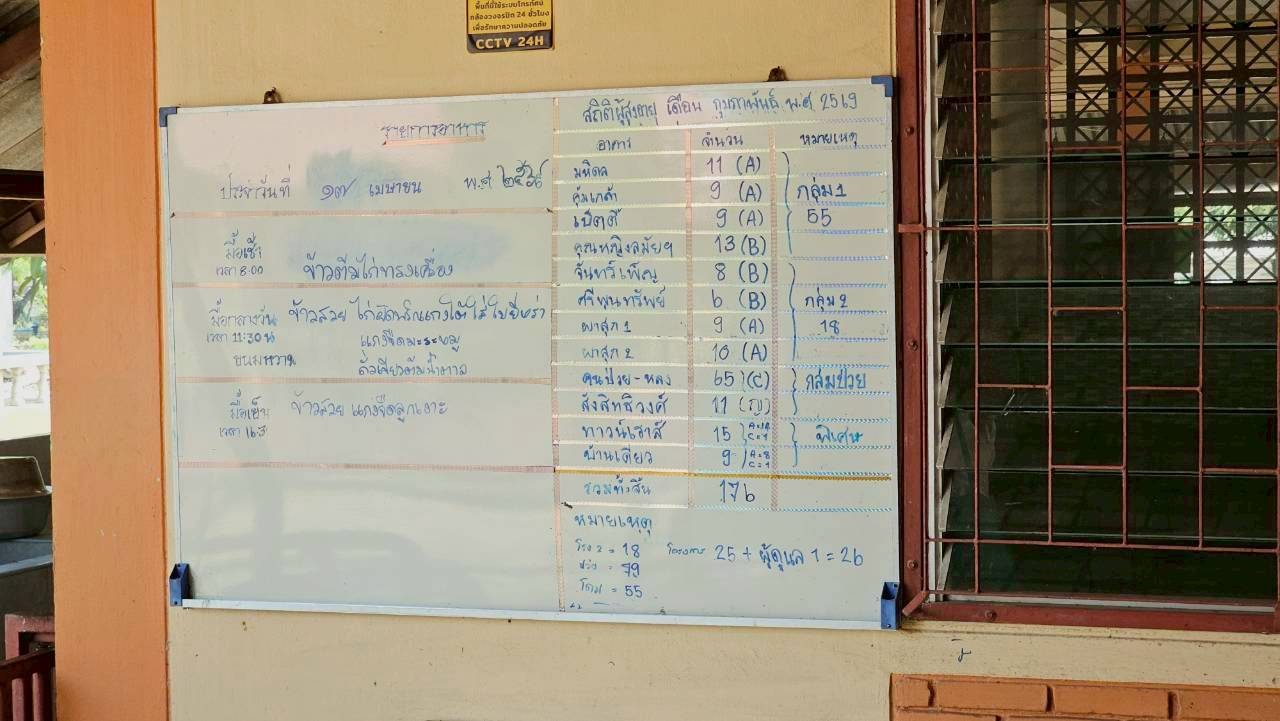
\includegraphics[width=\linewidth]{assets/appendices/legacy-field/workflow-board-1.jpg}
        \caption{บอร์ดแนวคิดการทำงานชุดที่ 1}
    \end{subfigure}
    \hfill
    \begin{subfigure}[t]{0.48\textwidth}
        \centering
        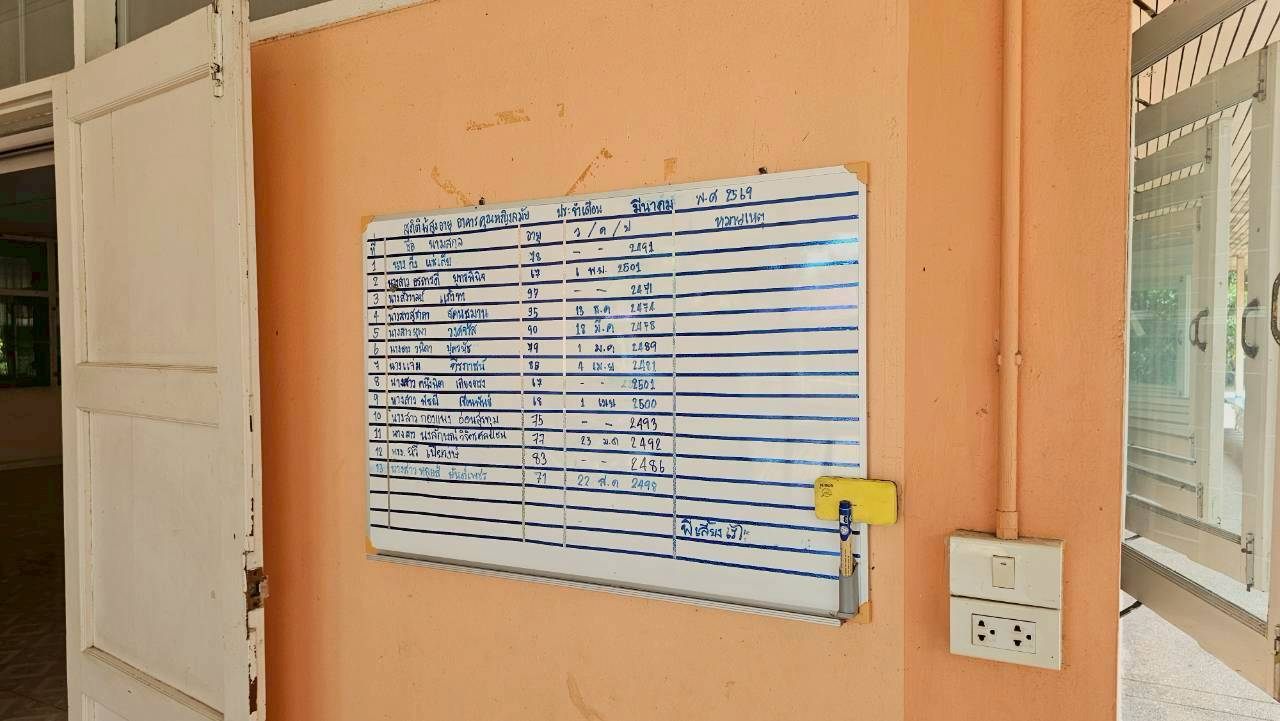
\includegraphics[width=\linewidth]{assets/appendices/legacy-field/workflow-board-2.jpg}
        \caption{บอร์ดแนวคิดการทำงานชุดที่ 2}
    \end{subfigure}
    \caption{ภาพประกอบการสรุปแนวคิดและ workflow ระหว่างการออกแบบระบบ}
    \label{fig:appI_workflow_boards}
\end{figure}

\begin{figure}[H]
    \centering
    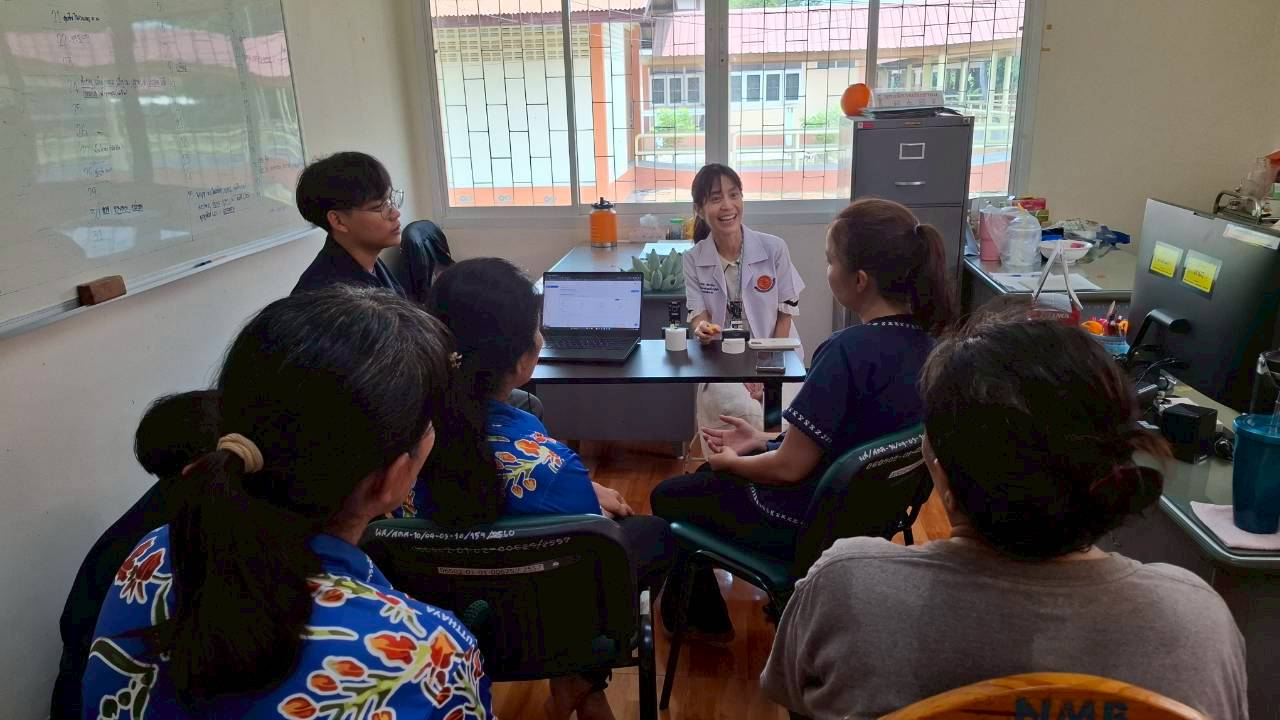
\includegraphics[width=0.82\textwidth]{assets/appendices/legacy-field/caregiver-feedback.jpg}
    \caption{ตัวอย่างการอธิบายแนวทางใช้งานระบบและรับฟังความคิดเห็นจากผู้ดูแล}
    \label{fig:appI_caregiver_feedback}
\end{figure}

\begin{figure}[H]
    \centering
    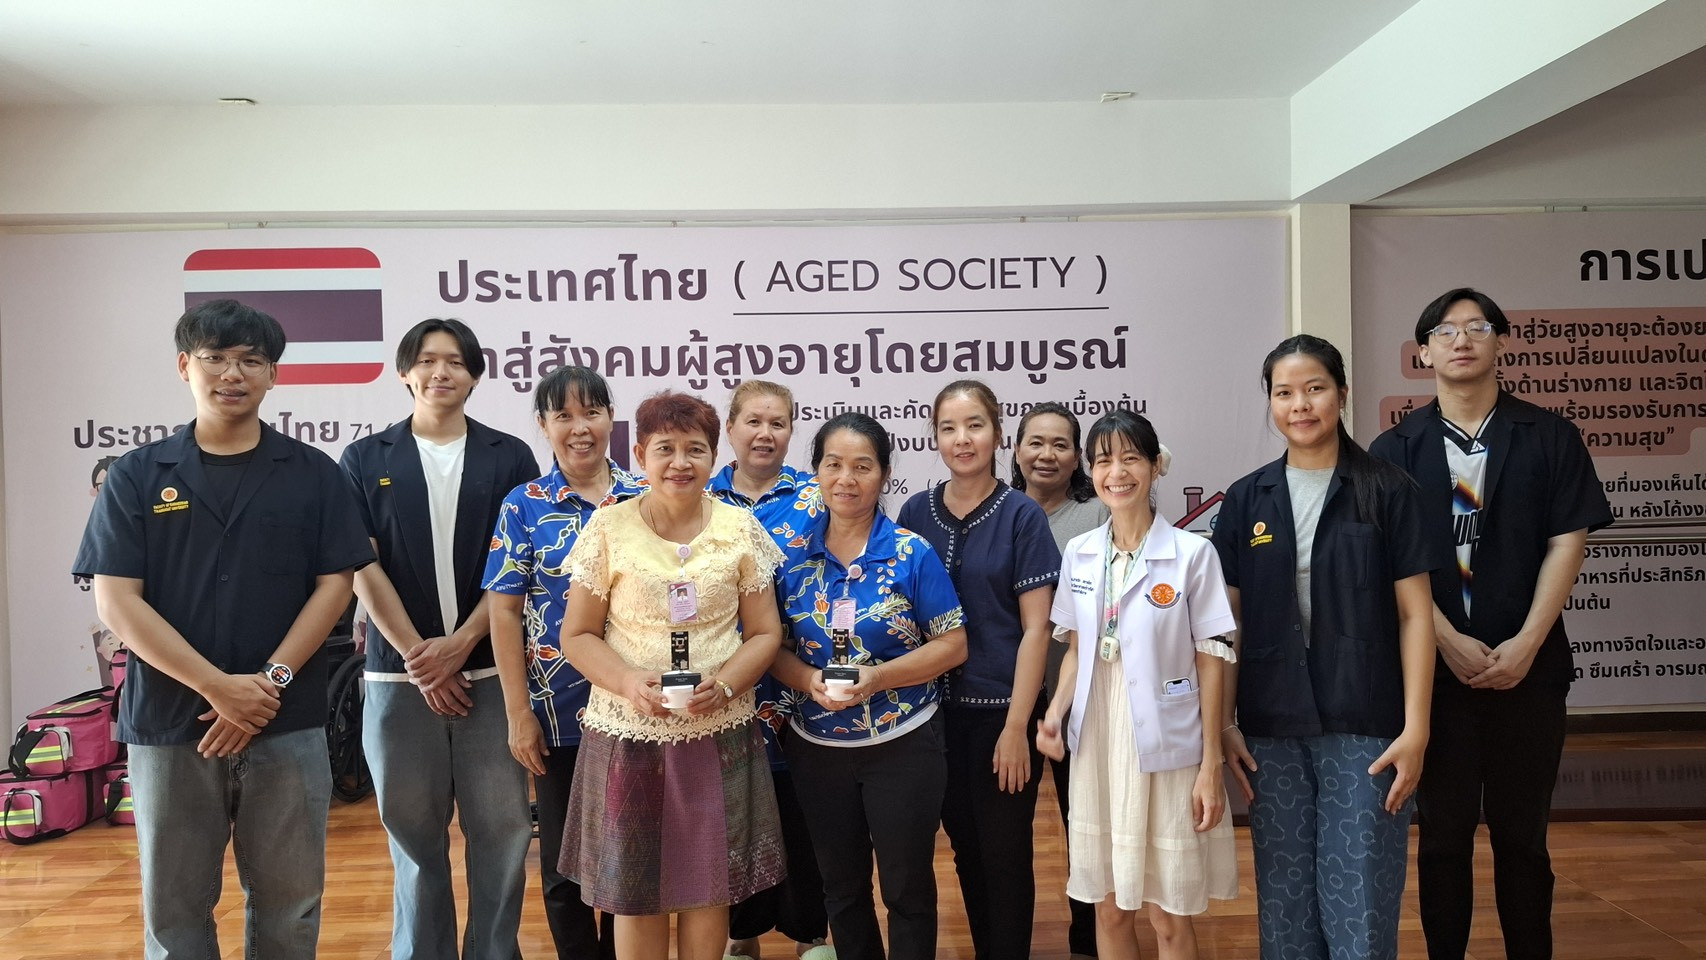
\includegraphics[width=0.82\textwidth]{assets/appendices/legacy-field/group-photo.jpg}
    \caption{ภาพประกอบการลงพื้นที่และการพูดคุยกับผู้เกี่ยวข้อง}
    \label{fig:appI_group_photo}
\end{figure}
